%!TEX root = dissertation.tex
%%%%%%%%%%%%%%%%%%%%%%%%%%%%%%%%%%%%%%%%%%%%%%%%%%%%%%%%%%%%%%%%%%%%%%%%%%%%%%%
\chapter{Introduction}

%% new thesis stuff
Packet Switching is the process of chunking information into smaller bits, labeling it and transmitting it independently. Paul Baran described this process in the 1960s\cite{baran1964distributed}. It changed a lot and provided one of the foundations for the emergence of the Internet. ARPANET, evolution, today's scale, outside and inside developments brings new Internet usage (mp3+p2p, bandwidth+codecs -> video, digicams/camcorder), mobile networks: more of a parallel development to the Internet, started from the old copper/telephony/circuit switched world, very slow development compared to Internet (in the beginning), but now finally able to do stuff, HOWEVER, very different beast, circuit switched roots, signalling, explicitly NOT a distributed system as compared to Internet, i.e. explicit signalling central controllers; now let's do research on it


%% old
The Internet began its life in the 1960s after the invention of packet switching \cite{baran1964distributed}. Throughout the years an amalgamation of networks, protocols, architectural evolutions, constant and changing principles, and applications lead to the Internet in its current form.

Today, services based on the World Wide Web dominate the Internet's landscape. Especially noteworthy is the dominance of video streaming services in the traffic mixes of today and in future predictions (cf. Figures fig:netvine and fig:cisco). This development was supported through the availability of cheap and small digital camcorders and especially the now sufficient access bandwidth to support high quality video streams.
A similar development for cellular networks is now ongoing. Through the advent of affordable high performance smartphones and access technologies like UMTS and LTE many are now using their phones as the primary device for interacting with the Internet, including video streaming services such as YouTube, Netflix, or Hulu.

\begin{figure}
	\centering
    	\begin{subfigure}[b]{0.50\textwidth}
                \centering
                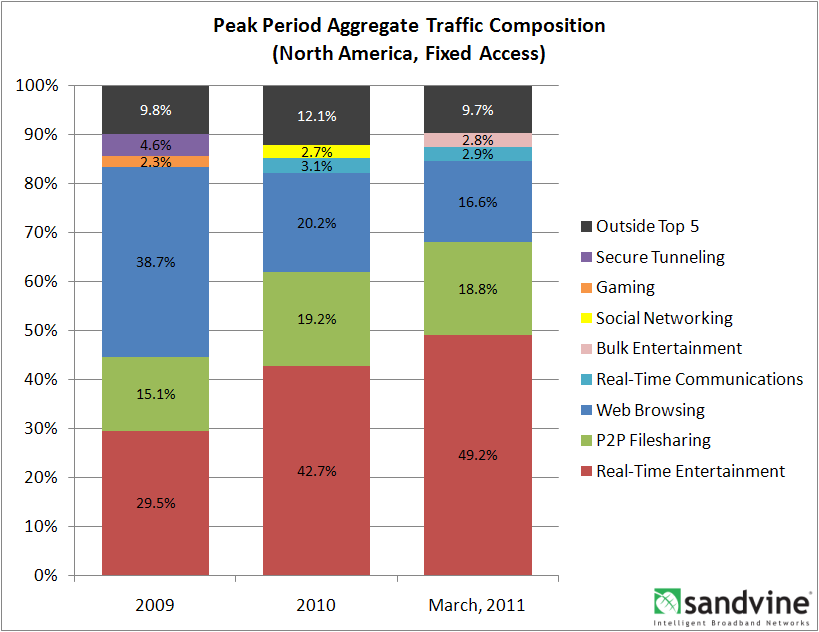
\includegraphics[width=\textwidth]{images/expose/netvine.png}
                \caption{Netvine, North American peak traffic (Source: \cite{sandvine_spring2011}).}
                \label{fig:netvine}
        \end{subfigure}%
        ~
    	\begin{subfigure}[b]{0.50\textwidth}
                \centering
                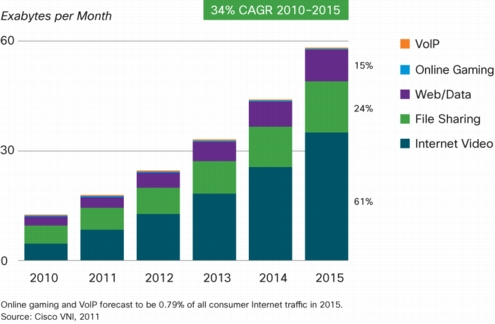
\includegraphics[width=\textwidth]{images/expose/ciscoVNI.jpg}
                \caption{Cisco, global consumer Internet traffic prediction (Source: \cite{cisco2011VNI}).}
                \label{fig:cisco}
        \end{subfigure}
	\caption{Traffic measurements and predictions.}
	\label{fig:traffic}
\end{figure}


This can put pressure on the overly complex cellular network structures. The radio transmissions have only access to a limited radio frequency spectrum that, moreover, has to be shared with any other phone user in the same cell. But there is also deemed to be significant pressure on the traffic management mechanisms of the mobile core networks backing up and aggregating the numerous radio cells of an operator. Little is known of the exact make-up of these networks as they are closely guarded secrets of the operator.

The popularity of these video services can to a degree be attributed to their full integration into the WWW. While previous offerings used completely different techniques which required the use of additional software, today one can enjoy videos just by directing ones browser to a website. Furthermore, other services related to video streaming are now also beginning to migrate to Web platforms. An example that is becoming increasingly popular at the moment are cloud gaming offerings which uses mechanisms very similar to real time video streaming but has stringent temporal constraints.


The topic of the thesis will be the research of the inner workings of these new streaming services and mechanisms and especially its impact on the aforementioned cellular core network structures. This means conducting performance evaluations of the streaming mechanisms on itself and in the context of mobile networks as well as performing systematic assessments and classifications of the mechanisms. 

The result will be an understanding of the quantitative attributes related to these new forms of streaming. Furthermore, the thesis should provide tools and methods that help decide all participants of media streaming and mobile network operators which protocols and methods to choose and which are best suited for specific applications.

The tackled protocols, systems, and mechanisms are described in Section X. Section Y details the methods that are and are planned to be used for the research. The final section gives a rough estimation on the thesis' schedule.


%TODO:
%Thesis' Future Impact
%    Performance analysis and comparison model of existing media streaming solutions
%      But do not compare the protocols but the mechanisms and paradigms behind it
%    Special focus on mobile environments and their pitfalls
%    Improvements to protocols and new approaches


%Concepts for future Internet structures are strongly disputed at the moment. A vast array of concepts is under discussion to either replace or enhance the protocol stack of the Internet's current setup. It will be interesting to measure the influence on media streaming and transport of these proposed changes or if there is any influence at all.

    
    %Neue Videostreamingtechniken sind beliebt und bringen immer mehr Last in Mobilfunksysteme. Die Leistungsfähigkeit und die Qualität der Streaming-Dienste hängt insbesondere vom Verkehrsmanagement in Mobilfunksystem ab. Die Arbeit soll die Leistungsfähigkeit der neuen Streamingverfahren in heutigen und zukünftigen Mobilfunksystemen, die mit dem Internet verbunden sind, untersuchen. Die Schwierigkeit der Arbeit besteht in der Komplexität der Mobilfunksysteme und der neuen Streamingverfahren sowie in der Verknüpfungen der beiden Konzepte. Insbesondere die Auswirkung der Mobilfunkkernnetze auf die Leistungsfähigkeit der Mechanismen der Transportschicht sollen mit Hilfe von Methoden aus der Leistungsbewertung von Rechner- und Kommunikationsnetzen, untersucht werden.







%It was originally used to enable login to remote computers and soon thereafter remotely accessing files using FTP. But from it emerged countless other services and applications that are today used by hundreds of millions of people touching almost every aspect of daily life. 

%The rise of the World Wide Web in the 1990s and even more in the last years made adoption of the Internet for the masses much easier. One needs just a single application to access and participate in most of the Internet's content in an easy accessible viewing format, i.e. the Web page defined with HTML.

%External influences and developments also had a huge impact on the development of the Internet and the Web. E.g. it can be argued that the invention of MP3 audio compression lead to the development of peer-to-peer mechanisms and file sharing (Napster). The wide spread of digital cameras and camcorders was one of the pillars of success for social networks, including video streaming sites like YouTube.
%A further requirements for these were the ever-increasing bandwidth capacities users had to access the Internet creating a two-way feedback loop. For every leap in bandwidth new services came up that filled it and fuelling the users' demand for further capacity increases. 

%Several factors contributed to the quick acceptance of the Internet. On the one hand, there are no assumptions made on the transported content. In contrast to the circuit switched telephone networks, which favor one mode of transportation and content (voice calls with specific procedures and/or codecs), in the Internet every packet is treated in the same way, leveling the playing field for every contender. On the other hand, one of the driving concepts of the Internet is the "End-to-End Principle" \cite{saltzer1984end2end, bhattacharjee1997active, blumenthal2001rethinking, isenberg1997rise, lemley2000end} which states:

%''The function in question can completely and correctly be implemented only with the knowledge and help of the application standing at the endpoints of the communications system. Therefore, providing that questioned function as a feature of the communication system itself is not possible. (Sometimes an incomplete version of the function provided by the communication system may be useful as a performance enhancement)'' \cite{saltzer1984end2end} 

%This means, that functionality, i.e. services or applications, should only be implemented at the two endpoints of any packet flow. Making assumptions of the higher protocol layers and implementing functions in the network, essentially making it intelligent, will always only be valid for existing and narrow use cases and cannot support future developments. Despite critical arguments, e.g. in \cite{reed2000endofe2e, moors2002critical}, and mechanisms that superficially seem to violate it (NAT, ECN) this principle still drives progress in the Web.

%The total volume if of Internet traffic has for many years been rising exponentially, as stated often fueled through external developments. The composition of today's traffic is manifold, but one large contributing factor is video. 
%Video transport in the Internet is currently a topic of hot discussions. Older and well researched transport modes, e.g. RTP, are challenged by new ones, which integrate themselves better into the current web ecosystem. Yet, they use completely different approaches to streaming and the control thereof. This is also the first research interest of the doctoral thesis.
%Streaming, or more generalized media transport is also not only relevant for the purpose of watching videos, there are many more fields of use which have slightly different requirements. With the popular cloud computing approach, which essentially means to run ones applications remotely on any number of hosts, it is necessary to transport the output of the applications, which often can be graphical, to the client. This is especially true for so-called Cloud Gaming services, which have hard temporal constraints on both directions of the transport path.

%Mobile networks are still much closer to their circuit switching roots. Having evolved from GSM over UMTS to LTE, mobile networks have only very recently become fully packet switched. However, the data transport through its many core network elements is still using connection oriented techniques. The radio access' properties are also wildly different to traditional This poses unique challenges and opportunities for the design and performance of protocols. Therefore, we take a special interest in mobile network environments in our research of video streaming.

%Concepts for future Internet structures are strongly disputed at the moment. A vast array of concepts is under discussion to either replace or enhance the protocol stack of the Internet's current setup. It will be interesting to measure the influence on media streaming and transport of these proposed changes or if there is any influence at all.


%TODO:
%Thesis' Future Impact
%    Performance analysis and comparison model of existing media streaming solutions
%      But do not compare the protocols but the mechanisms and paradigms behind it
%    Special focus on mobile environments and their pitfalls
%    Improvements to protocols and new approaches


%\begin{itemize}
%  \item The Internet
%    \begin{itemize}
%      \item Setup and Principles
%      
%        History, ARPA, setup, AS, (interdomain) routing
%        
%        remote login, FTP, WWW, real time, streaming, P2P, influence of external developments, issues
%        
%        end-to-end principle
%        
%        content agnosticism: we do not know what applications the future will bring, so we do not make any assumptions
%        
%      \item The World Wide Web on Top of the Internet
%        History, technical makeup
%      
%      \item Future Internet and/or the Future of the Internet
%        Near and long-term, IPv6, open access, bit pipes, critical review of arguments, end-to-end principle, Voluntary and indirect network assistance, moving functionality up the layer, quality of service and/or network neutrality
%    \end{itemize}
%    
%    
%  \item Streaming and Other Transmission Approaches
%    History, correlation to external developments (codecs, access bandwidths), techniques
%    
%    Why HTTP streaming? Generalization of HTTP streaming (reliable transport, control shift to the client)
%    
%  \item Mobile Access Technologies
%    GSM, UMTS, LTE, circuit and packet switching, mobility, issues, mobile network setup
%    
%    LTE and EPC makeup, tunneling backend approach
%    
%    Special requirements and convergence


%  \item Thesis' Future Impact
%    Performance analysis and comparison model of existing media streaming solutions
%      But do not compare the protocols but the mechanisms and paradigms behind it
%    Special focus on mobile environments and their pitfalls
%    Improvements to protocols and new approaches

%\end{itemize}
%%%%%%%%%%%%%%%%%%%%%%%%%%%%%%%%%%%%%%%%%%%%%%%%%%%%%%%%%%%%%%%%%%%%%%%%%%%%%%%%
%\subsection{The Internet: Setup and Principles}
%History, ARPA, setup, AS, (interdomain) routing


%%%%%%%%%%%%%%%%%%%%%%%%%%%%%%%%%%%%%%%%%%%%%%%%%%%%%%%%%%%%%%%%%%%%%%%%%%%%%%%%
%\subsection{Future Growth, Innovation, Changing and Constant Principles}
%remote login, FTP, WWW, real time, streaming, P2P, influence of external developments, issues


%Centrifugal approach. Decentralization. User empowerment 
%socioeconomic developments of a free speech network


%Whole is bigger than the sum of its parts. Protocols may not be best suited for every task

%Evolving technologies through bandwidth overhead. Things that were not thought possible only a few years back are now common practice
%-> High Frequency Trading
%-> Multimedia
%-> Real-Time VoIP Video
%-> BitCoin

%New traffic patterns emerging due to external developments. Digital cameras, new codecs (esp MP3, mpeg4, WebM) -> p2p, Webcams 


%%%%%%%%%%%%%%%%%%%%%%%%%%%%%%%%%%%%%%%%%%%%%%%%%%%%%%%%%%%%%%%%%%%%%%%%%%%%%%%%
%\subsection{Future Internet and/or the Future of the Internet}
%Near and long-term, IPv6, open access, bit pipes, critical review of arguments, end-to-end principle, Voluntary and indirect network assistance, moving functionality up the layer, quality of service and/or network neutrality

%all approaches lack proof why current Internet will not work anymore

%Open Access and FTTH

%End-to-end arguments in system design \cite{saltzer1984end2end}

%The End of End to End \cite{reed2000endofe2e}

%A critical review of end-to-end arguments in system design \cite{moors2002critical}

%Active networking and the end-to-end argument \cite{bhattacharjee1997active}

%Rethinking the design of the Internet: the end-to-end arguments vs. the brave new world \cite{blumenthal2001rethinking} : end-to-end enables the freedom to innovate and puts the choice of software and services completely to the user, no assumptions of the network have to be made
%"[...] when are actions of an ISP responsible management, and when are they manipulative control of the nature and effective pricing of content and application?"

%Rise of the stupid network \cite{isenberg1997rise}

%Moore's Law \cite{moore1998cramming} stronger than ever (doubling every ~14 months)


%%%%%%%%%%%%%%%%%%%%%%%%%%%%%%%%%%%%%%%%%%%%%%%%%%%%%%%%%%%%%%%%%%%%%%%%%%%%%%%%
%\subsection{The World Wide Web on Top of the Internet}
%History, technical makeup
%Why it works so well.

%"The Web adopts relatively simple technologies with sufficient scalability efficiency and utility" \cite{W3Arch}


%\subsection{Streaming and Other Transmission Approaches}
%History, correlation to external developments (codecs, access bandwidths), techniques

%%%%%%%%%%%%%%%%%%%%%%%%%%%%%%%%%%%%%%%%%%%%%%%%%%%%%%%%%%%%%%%%%%%%%%%%%%%%%%%%

%\subsection{Mobile Access Technologies}
%GSM, UMTS, LTE, circuit and packet switching, mobility, issues, mobile network setup
%The Internet is ubiquitous. 



%Baran packet switchting

% Less control, more effective
% Why global QoS control doesn't work.


%network intelligence at the end nodes
%End-to-end principle 
%Saltzer et al. ''The function in question can completely and correctly be implemented only with the knowledge and help of the application standing at the endpoints of the communications system. Therefore, providing that questioned function as a feature of the communication system itself is not possible. (Sometimes an incomplete version of the function provided by the communication system may be useful as a performance enhancement)'' \cite{saltzer1984end2end} 
% --> end-to-end violations: ECN? only signaling, decision is e2e, same category as indirect TCP congestion control signaling (through loss) from the network
%                            NAT, Firewalls?
%Authors' 2000 followup \cite{reed2000endofe2e}
%critical article \cite{moors2002critical}

% Not moving out of the box but instead exploring the dimensions of and improving the box itself


%layered model: application/intelligence always in the host; no distinction between hosts (be it user or network company); drives innovation

%dual use technology


% providers as bitpipes: layered model and end-to-end principle restricts providers to commodity business, similar to electricity providers; competition happens at the edge

%There's also the most controversial notion of a ,,future internet''. What this essentially means is ditching the whole hardware and software of the Internet and replacing it with a clean slate more managed designed protocol suit (yet ignoring why the Internet is successful). It is up to the thesis to decide, whether such an questionable endeavor is justified.

% IPv6
% Mobile L1/L2 differences, interference with assumptions that Ethernet is used

% LTE, EPC, Core network tunneling concepts, bottlenecks in the access and the core, LTE network model


% Improvements to congestion control for mobile streaming


% Influence of L1/2/3 layer protocols and mechanisms (IPv4/6, tunneling, ethernet vs RLC/RRC/NAS, ...) ; what works better with it? compare, model and measure



%Paul Müller, define protocol stacks by features, assemble on the fly -> performance?

% SmoothIT mechanisms; lower layer elements provide information to higher layers, overlays  \cite{oechsner2009pushing}


%%%%%%%%%%%%%%%%%%%%%%%%%%%%%%%%%%%%%%%%%%%%%%%%%%%%%%%%%%%%%%%%%%%%%%%%%%%%%%%%
\section{Internet Services}


Most of today's services base itself on the Web and HTTP as ``transport protocol''. It is even proposed to use
a slightly modified version of HTTP as the basic end-to-end protocol for a future iteration of the Internet\cite{Popa:2010:HNW:1868447.1868453} as it already fulfils many of the demands proposed for the future of the Internet.


There are other applications related to video streaming and are showing similar transmission characteristics. Examples include remote desktop services or cloud gaming. Cloud gaming facilitates the same core principles as video streaming. However, it adds strong bidirectional real time requirements as user interaction needs to be immediately reflected in the streamed images. One of the concerns of the thesis could be an investigation of streaming models for cloud gaming in the context of mechanisms used . Initial work has already been done, e.g., in \cite{4795441,wang2009modeling,jarschel2011cloudevaluation,ct2010wolken}.



%%%%%%%%%%%%%%%%%%%%%%%%%%%%%%%%%%%%%%%%%%%%%%%%%%%%%%%%%%%%%%%%%%%%%%%%%%%%%%%%
\section{Mobile Networks}



%%%%%%%%%%%%%%%%%%%%%%%%%%%%%%%%%%%%%%%%%%%%%%%%%%%%%%%%%%%%%%%%%%%%%%%%%%%%%%%%
\section{Related Research}

Video streaming touches many aspects of computer communication network research. They can be categorized in aspects touching on the one hand the service itself and on the other hand  the transport and underlying network. This chapter splits the topic roughly on a top-down layer approach. At first, modern video streaming applications and their mechanisms are presented. Afterwards, the streaming transport is discussed with a concluding section on the influences of wired and especially mobile network architectures.



%%%%%%%%%%%%%%%%%%%%%%%%%%%%%%%%%%%%%%%%%%%%%%%%%%%%%%%%%%%%%%%%%%%%%%%%%%%%%%%%
%\subsection{Services in the Internet}

%\subsubsection{Video Streaming}

%observe existing systems, e.g. YouTube \cite{metzger2011delivery}

%\subsubsection{Mechanisms}
%RTP, HTTP, adaptivity and reliability, application layer flow control, push and pull, fairness, segmentation
%\subsubsection{Quality Estimation and Modeling}
%QoE metrics, MOS, stalling time and buffering models, subjective and objective testing

%
%Cloud gaming as a media streaming application with strong real-time requirements \cite{4795441,wang2009modeling,jarschelevaluation,ct2010wolken}


%%%%%%%%%%%%%%%%%%%%%%%%%%%%%%%%%%%%%%%%%%%%%%%%%%%%%%%%%%%%%%%%%%%%%%%%%%%%%%%%
%\subsection{Current and Future Transport Developments}

%\begin{itemize}
%\item Improvements to congestion control for mobile streaming
%\item Alternative modes of transport (e.g. DCCP, ECN, ReECN, RED, Google's SPDY or new approaches)
%\item Influence of L1/2/3 layer protocols and mechanisms (IPv4/6, tunneling, ethernet vs RLC/RRC/NAS, ...) %; what works better with it? compare, model and measure

%\end{itemize}



%Paul Müller, define protocol stacks by features, assemble on the fly -> performance?

% SmoothIT mechanisms; lower layer elements provide information to higher layers, overlays  \cite{oechsner2009pushing}



%%%%%%%%%%%%%%%%%%%%%%%%%%%%%%%%%%%%%%%%%%%%%%%%%%%%%%%%%%%%%%%%%%%%%%%%%%%%%%%%
%\subsection{Architecture and Protocols}

%Mechanisms and protocols for the future of media streaming

%\begin{itemize}
%\item Compensation mechanisms for reliable transport
%\item Model and quality estimations for improvements to adaptive streaming
%\item End-to-end encryption and Authentication mechanisms (e.g.IPSec, DNSSEC, CurveCP) %(Daniel J. Bernstein)
%\item Modifications to and issues with TCP
%  \begin{itemize}
%  \item TCP buffer bloat
%  \item Initial window size (IW10, ...)
%  \item WebSockets as streaming transport \cite{w3c2011websockets} \cite{heise2011websockets}
%  \item WebRTC
%  \item Relevance of multicasting or similar techniques for streaming transport (real-time live vs. stored)
  
%  \item
%  \end{itemize}
%\item Service discovery and positioning (DNS modifications, CDNs, URIs, "networking named content")
%\item Mobile networks
%  \begin{itemize}
%    \item Loss Hiding and conflict with congestion control mechanisms
%    \item Shared media access, streaming with bandwidth/delay variations
%    \item Mobility issues
%      \begin{itemize}
%        \item Mobility as a delay and loss source and its influence
%        \item Investigation of mobility awareness and prediction techniques ("unassisted mobility")
%      \end{itemize}
%    \item future mobile networks
%      \begin{itemize}
%        \item Influence of control planes % Remove/Merge Control and User Plane
%        \item Influence of (core) network elements (or a reduction thereof)
%      \end{itemize}
%  \end{itemize}

%\end{itemize}


% TCP modifications for short-lived connections (e.g. initially ignore congestion avoidance and push a lot of data at once (google.com approach, Increasing TCP's Initial Window)) 
%IW10: better response time, still fair
% Link page: http://code.google.com/speed/protocols/tcpm-IW10.html


%Network Unassisted/Independent Mobility / Mobility Prediction API: When will the next handover occur, how much delay and bandwidth do i currently have? Can i complete oustanding transfers or should i reschedule them? Or, e.g., should i request a lower quality fragment? // Requirements: Stateless short to midtermed "Connections", high granularity of data "packets"
%--> "Mobility Awareness" (Andrea Hess / Lenaugasse) \cite{hummel2010mobilität} PMLAR (Predictive mobility and location-aware routing protocol in mobile ad hoc networks)



%Evaluate Multicast viability for streaming; but don't overestimate it's influence as it probably will not be applicable to most upcoming streaming cases: 
%no individually starting stored media streaming 
%no(or maybe?) \textbf{adaptive} live streaming (streams would need to adjust for every recipient)
%yes(?) non-adaptive pushed walled-garden tv streaming; most probably not the future of streaming
%related: TCP/reliable multicast problem stated in \cite{day2008patterns} page 334; no congestion/flow control

%http://en.wikipedia.org/wiki/Network_congestion
%http://en.wikipedia.org/wiki/TCP_global_synchronization




%%%%%%%%%%%%%%%%%%%%%%%%%%%%%%%%%%%%%%%%%%%%%%%%%%%%%%%%%%%%%%%%%%%%%%%%%%%%%%%%
\section{Outline}




\subsection{Technical Solution Spaces}


\begin{figure}
\centering
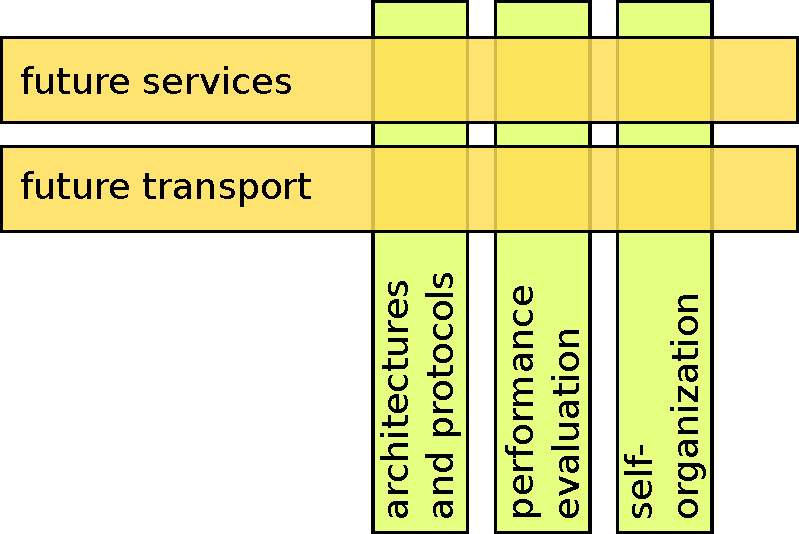
\includegraphics[width=0.4\textwidth]{images/expose/hv-topics-new.pdf}
\caption{Technical solution spaces to the problem layers.}
\label{fig:hv-topics}
\end{figure}

As discussed, the core problems are layered into services and transport. Technologically, to solve the tasks of video streaming, one can approach these  threefold as displayed in Fig. \ref{fig:hv-topics}.

The first is to dissect the involved protocols and architectures and break them down into their functional and methodical components. This will result in an improved understanding on the manner and process of their implementation. These components serve as building blocks for generalized models that abstracts the problem space from the actual implementation. The model will be defined by a set of parameters. To explore viable parameter ranges performance evaluation methods will be facilitated.


Secondly, using performance evaluation a system is methodically tested to the outcome of determining the influence of the system's parameters on a set of performance metrics. The parameters can be categorized into system intrinsic parameters, describing behavior only relevant and observable inside the system, and external parameters. In communication networks a good example for external parameters are the network Quality of Service parameters including latency, loss, jitter, and bandwidth capacity. Identifying fitting metrics for the measurement is a challenge. They can be either subjective or objective. The former are called Quality of Experience (QoE) metrics. They can only be measured by conducting empirical user studies and questionnaires and are mapped to a Mean Opinion Score (MOS). Extensive work has already been done to define baseline references for QoE metrics. Using these, one can directly translate objectively measurable outcomes into QoE metrics. However, these mappings may need to be adjusted to be able to handle stalling as the main source of quality loss. Examples for measuring subjective quality are available in \cite{gustafsson2008measuring, ketyo2010qoe}. 
Finally, one could employ methods of self-organization to try to reach improvements over conventional network setups.


\subsection{Apparatus for System Analyses and Comparison}

\begin{figure}[htbp]
\centering
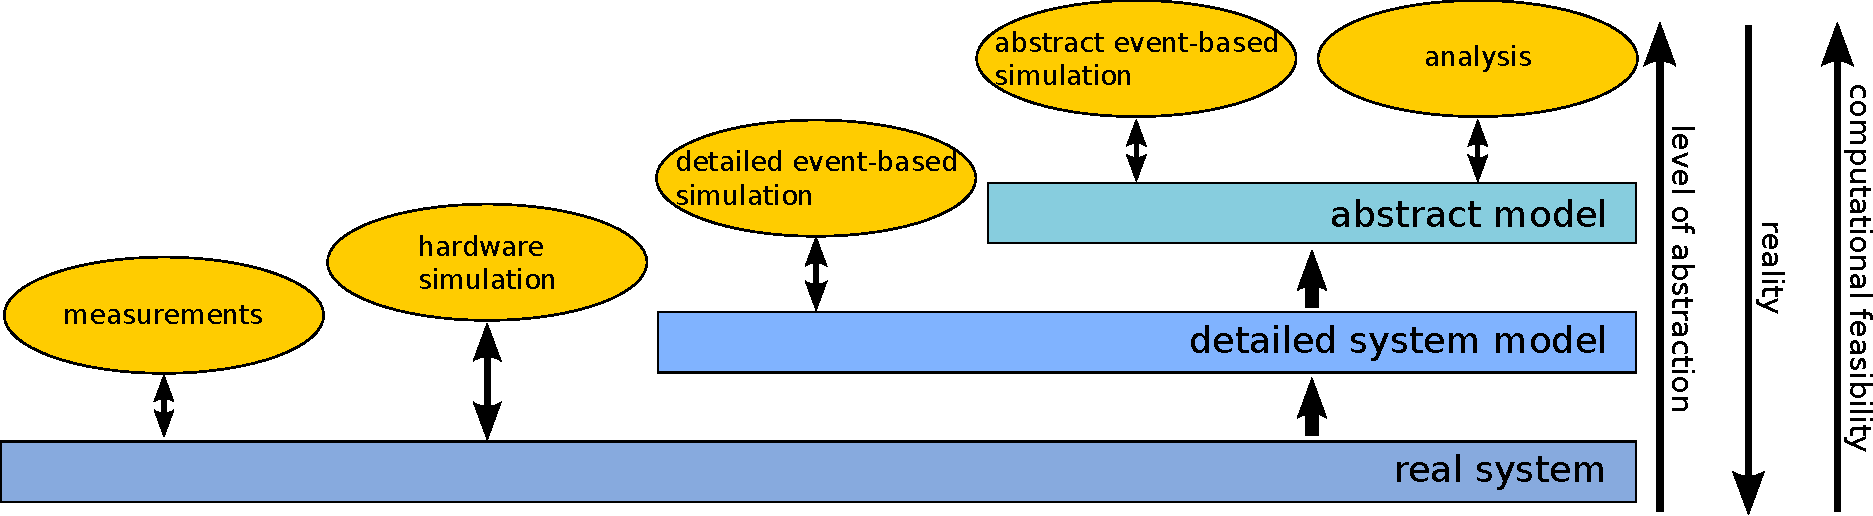
\includegraphics[width=1.0\textwidth]{images/expose/apparatus-new.pdf}
\caption{Methodical solution spaces and apparatus comparison.}
\label{fig:appcomp}
\end{figure}

Depicted in Figure \ref{fig:appcomp} are levels of abstraction involved in system analysis and possible approaches to understand the system involved.

The upper limit for precision is achieved through actual measurements of the system itself. These give a point of reference and can be used to validate all other methods. However, this is not feasible to ascertain a larger view. The time frame or the physical size of the system is always limited.

Aside from measurements on implementations there are three further possible approaches which can widen the scope: emulation, simulation and mathematical analysis. 
Emulation tries to resemble implemented functionality as closely as possible while reducing the non-important parts to a minimum. Measurements using emulations can run in a normal network environment testbed and thus can only be done on a scale equivalent to implementations. The simulative approach implements all internal and external functionality, including the physical nodes and the network, in a discrete event simulation (DES). There may be subtle functional differences between a simulation and a real implementation. Therefore, validation is required. This approach benefits from the decoupling of the simulation from physical nodes as well as real time, allowing to measure large-scale networks in a short amount of time.
A mathematical analysis, for example using queuing theory and stochastic models, can then further broaden the understanding of the system.


The methods can all be used to define and explore solution spaces and are therefore important tools in understanding the problem. A fitting combination of these tools has to be found to advance the research. Our initial approach is to investigate existing streaming services, YouTube \cite{metzger2011delivery,mok2011measuring} and,e.g., video libraries of broadcast stations for simple HTTP streaming. A suitable candidate for measuring adaptive streaming still needs to be found as some candidate services apply regional restrictions. There are several reference applications available that implement different standardization approaches. These can be used to either directly measure the performance or to setup an emulation model based on their specifications.


%\subsection{Further Approaches}
%Further approaches which are under consideration, but will not be presented in detail here, are:

%\begin{itemize}
%\item Application of analytic and stochastic methods.
%\item Formal definition of protocols or systems using Finite State Machines (FSM).
%\item Creation of equivalent models.
%\item Application of queuing theory, modeling the system through arrival processes, service time distributions and a number of servers and waiting places.
%\item Data-mining of network trace data from mobile networks.
%\end{itemize}


  
\subsection{Modeling Example for the Case of YouTube Streaming}

To give an example of the thesis' planned work an exemplary overview on the modelling process is presented. It was conducted for the buffering involved in YouTube's mode of streaming \cite{metzger2011delivery}. As YouTube uses a single-command pull-based approach for streaming, the influence the client has on the playback process is minimal. The player needs to maintain a tight control scheme on the playback buffer to accomplish as few buffer underruns as possible. The parameters that can be influenced by the player are: 

\begin{itemize}
\item Initial playback start delay.
\item Condition and timing for resuming playback after a buffer underrun occurs.
\end{itemize}

The constraints and metrics that must be achieved and can be observed:

\begin{itemize}
\item Maximum allotted buffer space at the client.
\item Subjective: Perceived quality of the playback process.
\item Objective: total and initial stalling times, frequency of interruptions.
\end{itemize}

External influences that were subjected on the model candidates to test their viability:

\begin{itemize}
\item Packet loss
\item Transmission latency
\end{itemize}

During the test, four specific models were formulated. These are:

\begin{enumerate}
\item \textit{Simple playback stalling}. Whenever anything can be played from the buffer do so. This results in the lowest required buffer space and also a lower limit for the total stalling time. However, it does not keep a safety buffer to handle insufficient connection quality, and is therefore prone to frequent micro-stalls.


\item \textit{Initial playback delay}. Delay the initial start until the video can be played without buffer underruns. It also acts as a lower limit for buffer space and total stalling time but additionally has the lowest frequency of stalls -- precisely one initial stall. It exhibits the best-case scenario for perceived quality disregarding the initial delay. However, it can not be implemented as an online algorithm, as it requires global knowledge.


\item \textit{Firefox HTML5}. The algorithm is depicted in Alg. \ref{alg:firefox}, its variables in Table \ref{tab:buffvars}. It does not differentiate between intermittent and initial conditions. The approach is in concept similar to the theoretical initial playback delay but results in very large required maximum buffer space due to conservatively chosen buffering times.

\begin{algorithm}
\centering
\caption{Firefox playback (re-)start decision algorithm.}
\label{alg:firefox}
\begin{algorithmic}
\IF {$s_{MA} > v_{MA}$} 
  \STATE $c \gets ( b_b=20s \lor b_T=20s )$
\ELSE
  \STATE $c \gets ( b_b=30s \lor b_T=30s )$
\ENDIF 
\end{algorithmic}
\end{algorithm}

\begin{table}
\centering
\begin{tabular}{|c|c|} \hline
Variable & Explanation \\ \hline\hline
$s_{MA}$ & Moving average of the transmission speed. \\ \hline
$v_{MA}$ & Moving average of the video bitrate. \\ \hline
$c$   & Condition upon which to start/resume playback. \\ \hline
$b_b$    & Amount of video data the buffer contains. \\ \hline
$b_T$    & Amount of time spent in non-playing buffering state. \\ \hline
\end{tabular}
\caption{Variables involved in buffering decisions.}
\label{tab:buffvars}
\end{table}

\item \textit{YouTube Flash Player}. $b_{b,initial}=2s$, $b_{b,intermittent}=5s$. Assumes sufficient network conditions in the beginning requiring only a short initial playback delay. If the assumption does not hold and stalling does occur, it will buffer longer to keep the occurrence frequency down.
\end{enumerate}


\begin{figure}
% used yt-delay/hPUGNCIozp0_delay_100 2, spyder with matplotlib config patch
	\centering
    	\begin{subfigure}[b]{0.50\textwidth}
                \centering
                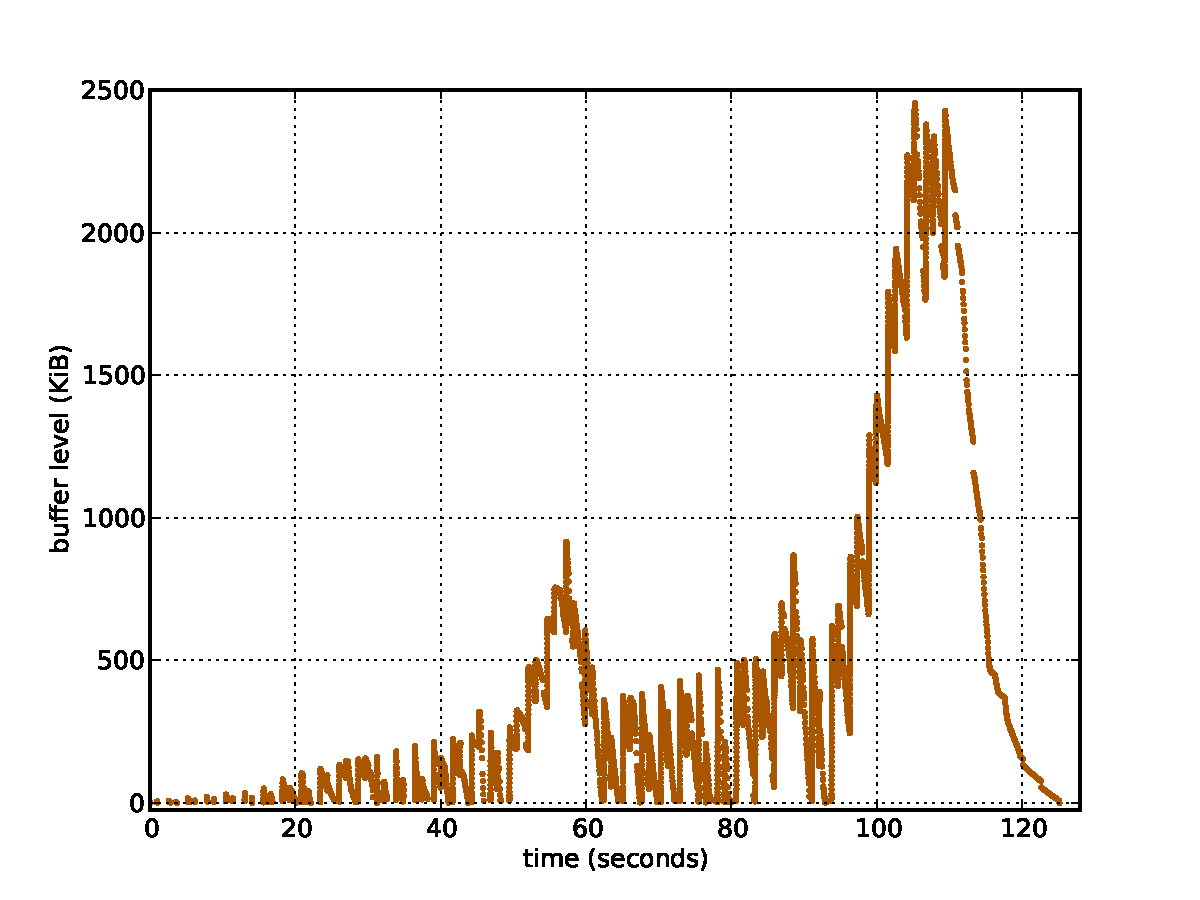
\includegraphics[width=\textwidth]{images/expose/bufferlevel-stall-new.pdf}
                \caption{Simple playback stalling method, 33s total stalling.}
                \label{fig:expose-bufferlevel-stall}
        \end{subfigure}%
        ~
    	\begin{subfigure}[b]{0.50\textwidth}
                \centering
                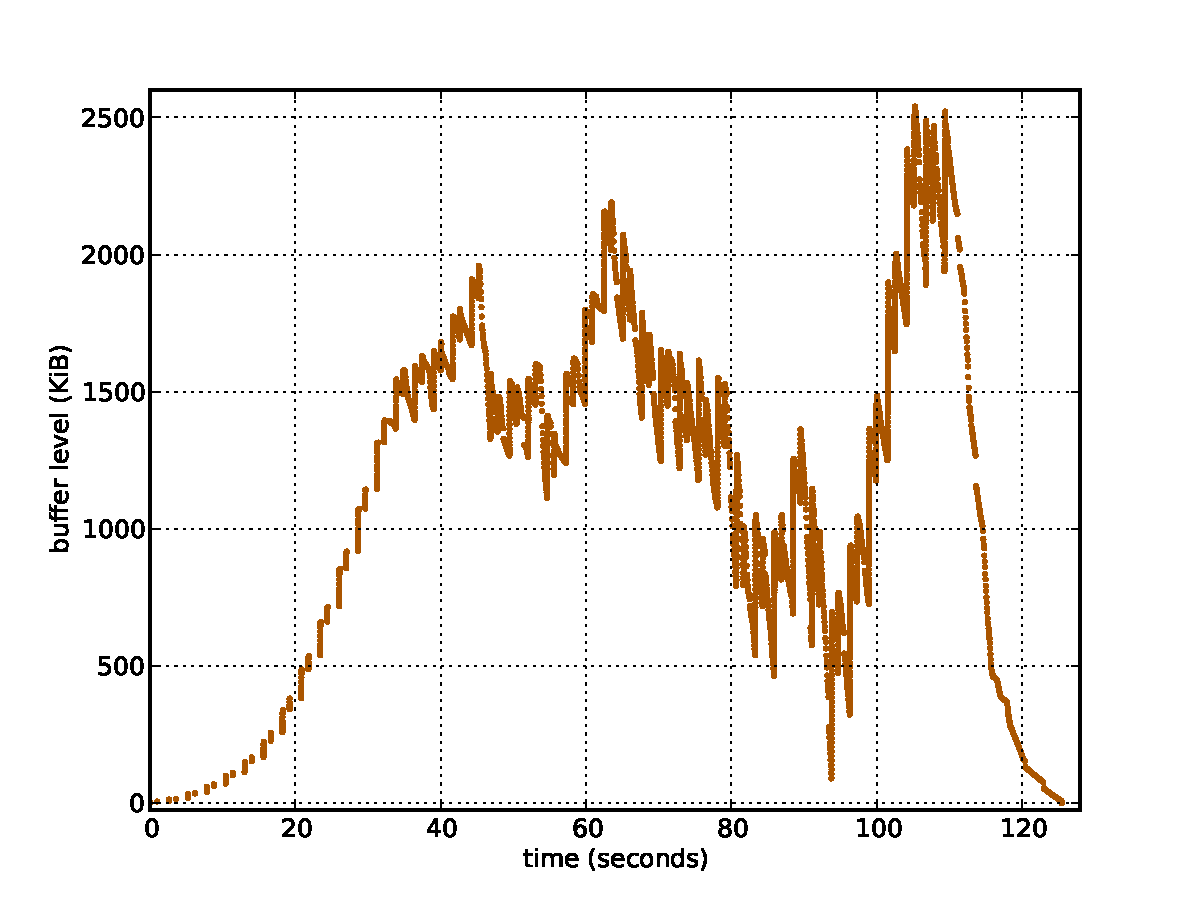
\includegraphics[width=\textwidth]{images/expose/bufferlevel-startdelay-new.pdf}
                \caption{Initial playback delay, 33s total stalling.}
                \label{fig:expose-bufferlevel-startdelay}
        \end{subfigure}

        \begin{subfigure}[b]{0.50\textwidth}
                \centering
                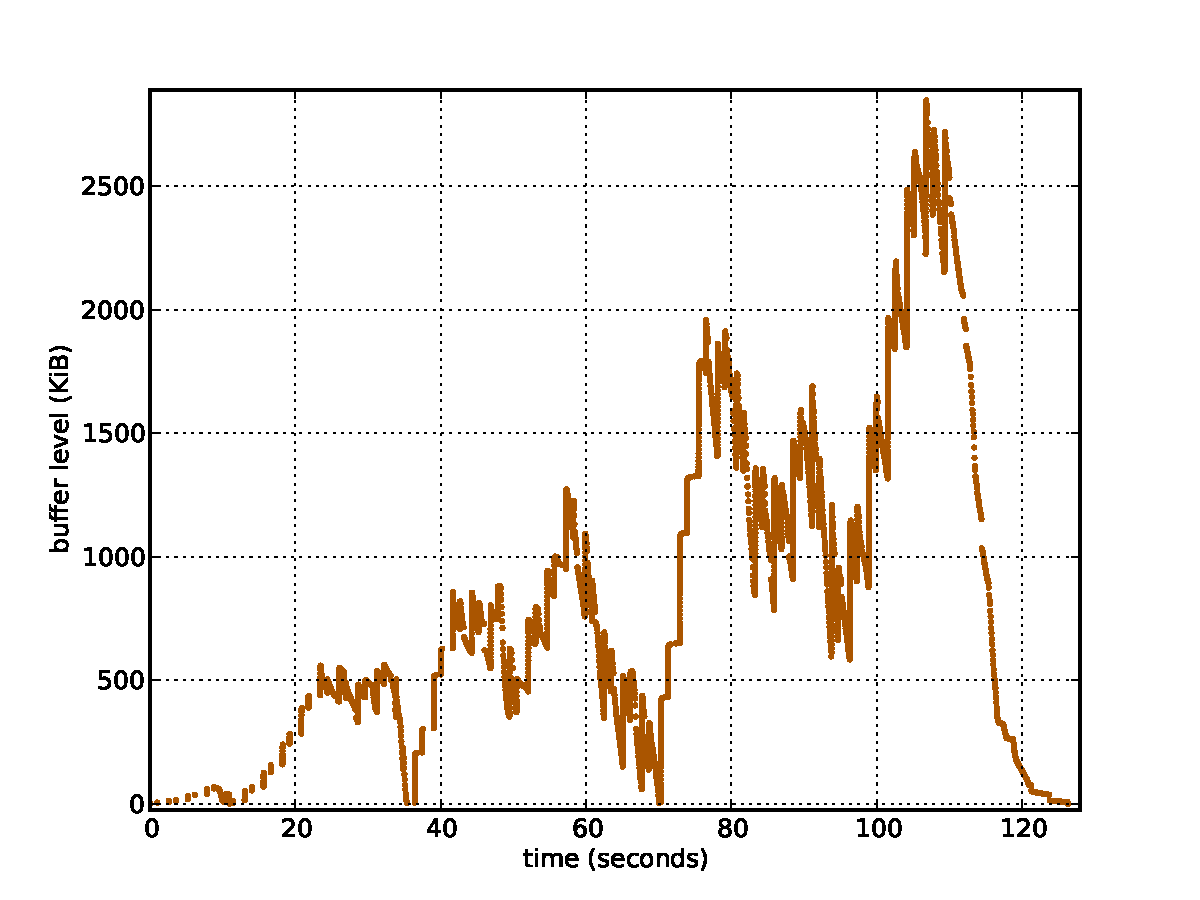
\includegraphics[width=\textwidth]{images/expose/bufferlevel-flash-new.pdf}
                \caption{YouTube Flash Player method, 34s total stalling.}
                \label{fig:expose-bufferlevel-flash}
        \end{subfigure}%
        ~
    	\begin{subfigure}[b]{0.50\textwidth}
                \centering
                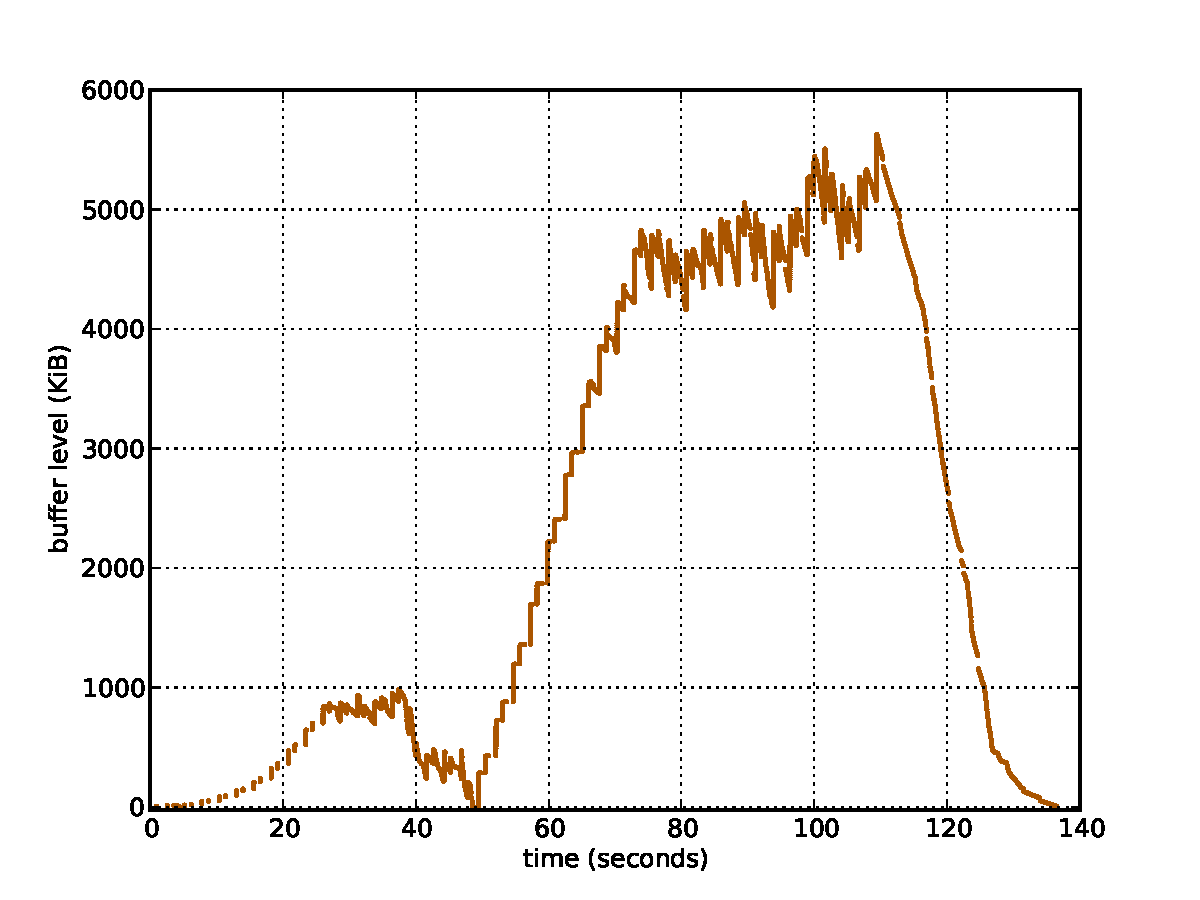
\includegraphics[width=\textwidth]{images/expose/bufferlevel-firefox-new.pdf}
                \caption{Firefox HTML5 method, 44s total stalling.}
                \label{fig:expose-bufferlevel-firefox}
        \end{subfigure}
	\caption{Modelled buffer fill level graphs and resulting total stalling times.}
	\label{fig:expose-bufferlevel}
\end{figure}


These models were compared with regards to the stalling frequency and duration in a test scenario. The resulting graphs are depicted in Figure \ref{fig:expose-bufferlevel}. Further research is now required to gather measurement data from several videos and QoS conditions to be able to make conclusions on the viability of the models.




As demonstrated, the ongoing work of this thesis is twofold, the application layer streaming and transport part and the mobile network component. Both can -- to some degree -- be tackled independently of each other. This is reflected in the thesis' proposed schedule in Table Z. When a sufficient understanding of both subtopics is reached one can then combine them and look at the bigger picture involved. Currently, work is being conducted on detailing the buffering behavior of simple HTTP streaming, partially already being published in \cite{metzger2011delivery}. Additionally, time is spent working on thematically overlapping ongoing projects.

The thesis should be concluded in the first or second quarter of 2014 with the last quarters being dedicated to the writeup and finalization work.


%Questions

%On which kind of network information flow should streaming applications rely on in general and mobile networks specifically? What information is actually required for streaming?

%What information flow should be provided by networks?

%How can and should information be exchanged?

%Can or should there be any dependence of the information flow on the application layer protocol?

%How can the information flow be evaluated and modelled and the protocols and network architectures be compared? Is a generic evaluation model possible?



%  \item Emulation and simulation
%  \item Performance evaluation
%\end{itemize}

%Design of new transport or streaming mechanisms
%-> Formal Description Techniques

%-> Analytical Tool, test viability

%\subsubsection{Mechanisms}

%\subsubsection{Quality Estimation and Modeling}
%QoE metrics, MOS, stalling time and buffering models, subjective and objective testing

%Creation of QoE models

